\documentclass[12pt]{article}
\usepackage[landscape,twocolumn]{geometry}% http://ctan.org/pkg/geometry
%------------------------------------------------------------------------------------------

% These commands will adjust the two column layout to look a bit better
% see: http://scholardox.com/pubs/Landscape.pdf
\usepackage{sectsty}
\setlength{\textheight}{17cm}
\setlength{\textwidth}{23cm}
\setlength{\topmargin}{-2.2cm}
\setlength{\oddsidemargin}{0.0cm}
\setlength{\evensidemargin}{\oddsidemargin}
\setlength{\parskip}{0cm}
\setlength{\columnsep}{1cm}
\sectionfont{\normalsize}
\subsectionfont{\normalsize}


%%------------------------------
%Make background the pdf "bkgd.pdf"
%\usepackage[pages=all]{background}
%\backgroundsetup{
%scale=1,
%color=black,
%opacity=1,
%angle=0,
%contents={%
%  \includegraphics[width=\paperwidth,height=\paperheight]{Resources/bkgd.pdf}
% }
%}

\usepackage{amsmath}
\usepackage{amssymb}
\usepackage{graphicx}
\usepackage[singlespacing]{setspace}
\usepackage{caption}
\usepackage{float}
\usepackage{pdfpages}
\usepackage{multicol}
\usepackage{gensymb}

\everymath{\displaystyle}

\usepackage{hyperref}%Make references, clickable links
\hypersetup{
    colorlinks,
    citecolor=black,
    filecolor=black,
    linkcolor=black,
    urlcolor=black
}


%------------------------------------------------------------------------------------------
\newcommand{\ei}{\vec{e_1}}   %e1 shortcut
\newcommand{\ej}{\vec{e_2}}   %e2 shortcut
\newcommand{\ek}{\vec{e_3}}   %e3 shortcut
\newcommand{\n}{\vec{n}}
\newcommand{\m}{\vec{m}}
\newcommand{\x}{\vec{x}}

\newcommand{\sig}{\sigma}       %sigma shortcut
\newcommand{\ep}{\varepsilon} %epsilon shotcut

\renewcommand{\vec}[1]{\mathbf{#1}} %make vectors bold


\newcommand{\beq}{\begin{equation}} %begin equation shortcut
\newcommand{\eeq}{\end{equation}} %end equation shortcut

\newcommand{\of}[1]{\left(#1\right)} %parenthases shortcuts
\newcommand{\ofa}[1]{\left[#1\right]} %brackets shotcut

%%------------------------------
\usepackage{empheq}
\usepackage[most]{tcolorbox}
% Box commands
\newtcbox{\mymath}[1][]{%
    nobeforeafter, math upper, tcbox raise base,
    enhanced, colframe=blue!30!black,
    colback=blue!30, boxrule=1pt,
    #1}

\newcommand{\pbox}[1]{\begin{empheq}[box=\mymath]{align*}#1\end{empheq}} %purple box shortcut

%------------------------------------------------------------------------------------------
%FANCY HEADER COMMANDS
\usepackage{fancyhdr}
%\pagestyle{fancy}
%\fancyhead[LO]{STRUCTURAL ANALYSIS}
\setlength{\headheight}{15.2pt}
\fancyhf{}
\lhead[STRUCTURAL ANALYSIS]{STRUCTURAL ANALYSIS}

%------------------------------------------------------------------------------------------
%TITLE PAGE COMMANDS
\title{Structural Analysis with the Direct Stiffness Method}
\author{Brian Chevalier}
\date{ \today }

%------------------------------------------------------------------------------------------
\begin{document}

\pagenumbering{arabic}
\makeatletter
\@twocolumnfalse
\maketitle
\@twocolumntrue
\makeatother
\vspace*{\fill}
\begin{center}
	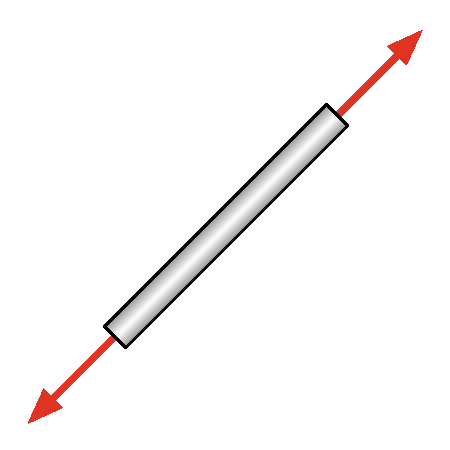
\includegraphics[scale=1]{Figures/Notesimg}
\end{center}
\vspace*{\fill}
\newpage

%------------------------------------------------------------------------------------------
\vspace*{\fill}
\begin{tcolorbox}[height=0.8\textheight, width=\columnwidth, colframe=gray, colback=lightgray, halign=left, arc=3mm]
	\tableofcontents
\end{tcolorbox}
\vspace*{\fill}

\newpage

\section{Truss Direct Stiffness Method}



%\includepdf[scale=0.8,pages=1,pagecommand=\section{Appendix A: MatLab Code}]{DOCUMENTTITLE}
%\includepdf[scale=0.8,pages=2-,pagecommand={}]{DOCUMENTTITLE}


%------------------------------------------------------------------------------------------
%\includepdf[scale=0.8,pages=1,pagecommand=\section{Appendix B: }]{DOCUMENTTITLE}
%\includepdf[scale=0.8,pages=2-,pagecommand={}]{DOCUMENTTITLE}


%------------------------------------------------------------------------------------------
\newpage
\bibliography{References}
\addcontentsline{toc}{section}{References}
\bibliographystyle{apalike}
%------------------------------------------------------------------------------------------

%----End of document
\end{document}